\section{Explaining the Phenomena of Negative Transfer in Multi-Task Learning}\label{sec_insight}

Based on Lemma \ref{lem_cov_shift_informal}, we rigorously explain the phenomena of negative transfer in multi-task learning.
We explain from three perspectives, including \textit{task similarity}, \textit{data size} and \textit{covariate shift}.
We show how negative transfer occurs as a result in a simplified model and describe the algorithmic consequence.

\subsection{Task Similarity}\label{sec_similarity}

It is well-known since the seminal work of Caruana \cite{C97} that how well multi-task learning performs depends on task relatedness.
We formalize this connection in the following simplified setting.

\textit{The isotropic model.}
	Consider two tasks with isotropic covariances $\Sigma_1 = \Sigma_2 = \id$.
	Recall that each task has data size $n_i = \rho_i \cdot p$, for $i = 1, 2$.
	And $X_1\in\real^{n_1\times p}, X_2\in\real^{n_2\times p}$ denotes the covariates of the two tasks, respectively.
	We assume that for the target task, $\beta_2$ has i.i.d. entries with mean zero and variance $\kappa^2$.
	For the source task, $\beta_1 $ equals $\beta_2$ plus i.i.d. entries with mean $0$ and variance $d^2$.
	The labels are given by $Y_i = X_i\beta_i + \varepsilon_i$, where $\e_i$ consists of i.i.d. entries with mean zero and variance $\sigma_i^2$, for $i=1,2$.
	We assume that all the random variables have subexponential decay, while keeping in mind that our results can be applied under weaker moments assumptions as shown in Appendix \ref{app_proof_sec3}.

In the isotropic model, we show that as we increase the distance between $\beta_1$ and $\beta_2$, there is a transition from positive transfer to negative transfer in MTL.
%We measure model dissimilarity as $\norm{\beta_1 - \beta_2}^2$, which is the distance between source and target in the isotropic model.
Figure \ref{fig_model_shift} provides a simulation when $p = 200$.
{The rest of parameter settings can be found in Appendix \ref{app_synthetic}.}
Our result below will provide an explanation to this phenomenon.
%Based on Theorem \ref{thm_model_shift}, we derive the transition threshold in the following proposition.
We introduce the following notations.
\begin{align*}
	\Psi(\beta_1, \beta_2) = {\ex{\bignorm{\beta_1 - \beta_2}^2}} / {\sigma^2},  \quad \Phi(\rho_1, \rho_2) = \frac{(\rho_1 + \rho_2 - 1)^2}{\rho_1 (\rho_1 + \rho_2) (\rho_2 - 1)}.
\end{align*}

\begin{proposition}[Task model distance]\label{prop_dist_transition}
	In the isotropic model, suppose that $\rho_1 > 1$ and $\sigma_1 = \sigma_2 = \sigma$.
	Then we have that
	%Whether $\te(\hat{\beta}_t^{\MTL})$ is lower than $\te(\hat{\beta}_t^{\STL})$ is determined by the ratio between $\Psi(\beta_1, \beta_2)$ and $\Phi(\rho_1, \rho_2)$:
	\squishlist
		\item If $\Psi(\beta_1, \beta_2) < \gamma_{-} \cdot \Phi(\rho_1, \rho_2)$, then w.h.p. over the randomness of $X_1,X_2$, $\te(\hat{\beta}_t^{\MTL}) < \te(\hat{\beta}_t^{\STL})$.
		\item If $\Psi(\beta_1, \beta_2) \ge \gamma_{+} \cdot \Phi(\rho_1, \rho_2)$, then w.h.p. over the randomness of $X_1,X_2$, $\te(\hat{\beta}_t^{\MTL}) \ge \te(\hat{\beta}_t^{\STL})$.
	\squishend
	Here $\gamma_{-} = (1-\oo(1))\cdot(1 - \rho_1^{-1/2})^4$ and $\gamma_{+} = (1+\oo(1))\cdot(1 + \rho_1^{-1/2})^4$.
	Concretely, if $\rho_1 > 40$, then $\gamma_{-} \in (1,2)$ and $\gamma_{+} \in (1/2, 1)$.
\end{proposition}

Proposition \ref{prop_dist_transition} simplifies Theorem \ref{thm_main_informal} in the isotropic model, allowing for a more explicit statement of the bias-variance tradeoff.
Concretely, $\Psi(\beta_1, \beta)$ and $\Phi(\rho_1, \rho_2)$ corresponds to $\Delta_{\bias}$ and $\Delta_{\vari}$, respectively.
Prosposition \ref{prop_dist_transition} explains the transition observed in Figure \ref{fig_model_shift}.
Note that there are several unexplained observations near the transition threshold $0$, which are caused by the concentration errors $\gamma_+, \gamma_-$.
%We fix the target task and vary the source task, in particular the parameter $d$ which determines $\norm{\beta_1 - \beta_2}$.
%Figure \ref{fig_model_shift} shows the result.
%We observe that Proposition \ref{prop_dist_transition} explains most of the observations in Figure \ref{fig_model_shift}.
%The proof of Proposition \ref{prop_dist_transition} involves two parts.
%First, in equation \eqref{eq_te_var}, the positive variance reduction effect scales with $n_1 = \rho_1 p$, the number of source task data points.
%Second, we show that the negative effect of model-shift bias scales with $pd^2$, which is the expectation of $\norm{\beta_1 - \beta_2}^2$.
The proof of Proposition \ref{prop_dist_transition} can be found in Appendix \ref{app_proof_31}. %, which is based on our main result described later in Theorem \ref{thm_model_shift}.

\begin{figure}
	\begin{subfigure}[b]{0.32\textwidth}
		\centering
		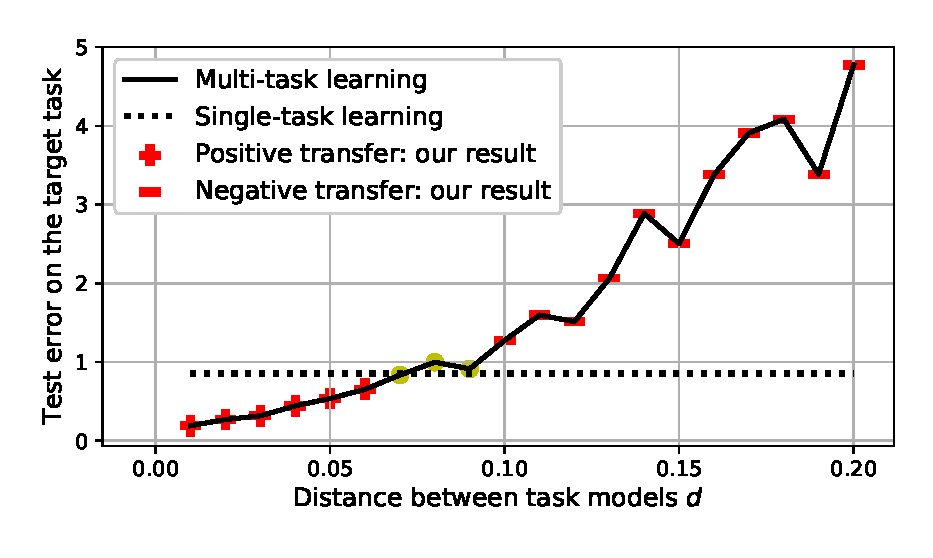
\includegraphics[width=0.98\textwidth]{figures/model_shift_phase_transition.eps}
		\caption{Task similarity}
		\label{fig_model_shift}
	\end{subfigure}\hfill
	\begin{subfigure}[b]{0.32\textwidth}
		\centering
		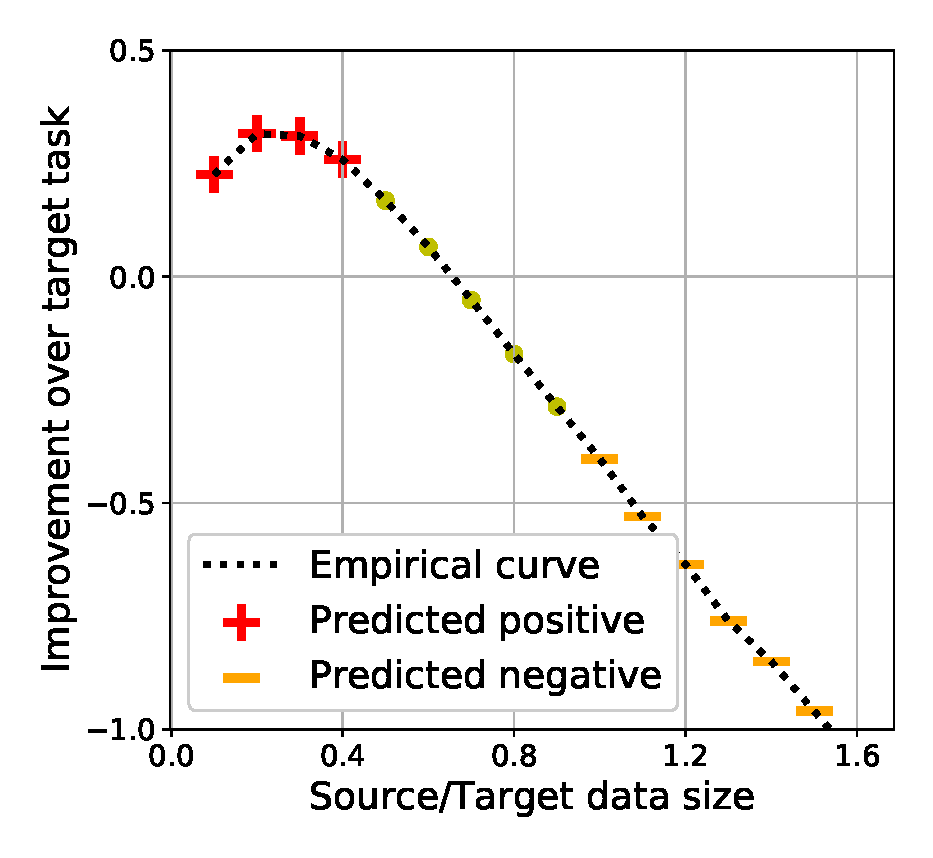
\includegraphics[width=0.98\textwidth]{figures/datapoints_phase_transition.eps}
		\caption{Data size}
		\label{fig_size}
	\end{subfigure}\hfill
	\begin{subfigure}[b]{0.32\textwidth}
		\centering
		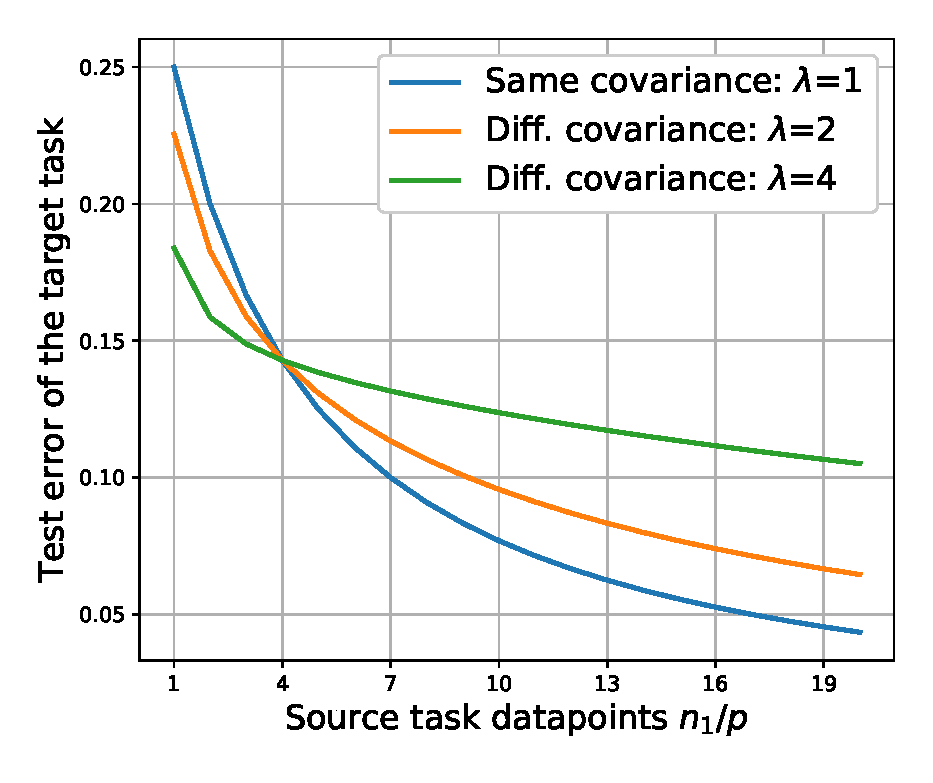
\includegraphics[width=0.98\textwidth]{figures/complementary.eps}
		\caption{Covariate shift}
		\label{fig_covariate}
	\end{subfigure}
	\caption{Three takeaways of our theory in Section \ref{sec_insight}.
	(a) As task model distance increases, we observe a transition from positive to negative transfer  (Proposition \ref{prop_dist_transition}).
	(b) As source/target data ratio increases, we observe a transition from positive to negative transfer (Proposition \ref{prop_data_size}).
	(c) As covariate shift gets more severe (measured by increasing $\lambda$), MTL performance gets worse (Proposition \ref{prop_covariate}).
	The $y$-axis measures the performance of MTL minus STL.}
	\label{fig_model_shift_phasetrans}
\end{figure}

\textbf{Algorithmic consequence.}
As an extension of Proposition \ref{prop_dist_transition}, we observe that MTL is particular powerful when the labeled data of the source task is less noisy compared to the target task.
Consider a more general setting of Proposition \ref{prop_dist_transition} where the noise level $\sigma_1$ of task $1$ differs from the noise level $\sigma_2$ of task $2$.
If $\sigma_1$ is too large, the source task provides a negative transfer to the target.
If $\sigma_1$ is small, the source task is more helpful.
We leave the result to the Appendix in Proposition \ref{prop_var_transition}.
Inspired by the observation, we propose a single-task based metric to help understand MTL results using STL results.
\squishlist
	\item For each task, we train a single-task model.
	Let $z_s$ and $z_t$ be the prediction accuracy of each task, respectively.
	Let $\tau\in(0, 1)$ be a fixed threshold.
	\item If $z_s - z_t > \tau$, then we predict that there will be positive transfer when combining the two tasks using MTL.
	If $z_s - z_t < -\tau$, then we predict negative transfer.
\squishend

\subsection{Data Size}\label{sec_data_size}

In classical Rademacher or VC based theory of multi-task learning, the generalization bounds are usually presented for settings where the data sizes are equal for all tasks \cite{B00,M06,MPR16}.
More generally, such results are still applicable when all task data are being added simultaneously.
On the other hand, for many applications of multi-task learning, the data sources are usually heterogeneous.
For such settings, we have observed that adding more labeled data from one task does not always help.
%On the other hand, we have observed that adding more labeled data does not always improve performance in multi-task learning.
Using the isotropic model, we consider what happens if we vary the source task data size.
Figure \ref{fig_size} provides a simulation result for such a setting.
We observe that as $n_1 / n_2$ increases, there is a transition from positive to negative transfer.
Our result below explains this phenomenon.

\begin{algorithm}[!t]
	\caption{An incremental training schedule for efficient multi-task learning with two tasks}
	\label{alg_inc_train}
	\begin{algorithmic}[1]
		\Input Two tasks $(X_1, Y_1)$ and $(X_2, Y_2)$.
		\Param A shared module $B$, output layers $W_1, W_2$ as in the hard parameter sharing architecture.
		\Req \# batches $S$, epochs $T$, task $2$'s validation accuracy $\hat{g}(B; W_2)$, a threshold $\tau\in(0,1)$.
		\Output The trained modules $B, W_2$ optimized for task $2$.
		\State Divide $(X_1, Y_1)$ randomly into $S$ batches: $(x^{(1)}, y^{(1)}), \dots, (x^{(S)}, y^{(S)})$.
		\For{$i = 1,\dots, S$}
			\For{$j = 1,\dots, T$}
				\State Update $B, W_1, W_2$ using the training data $\set{x^{(k)}, x^{(k)}}_{k=1}^i$ and  $(X_2, Y_2)$.
			\EndFor
			\State Let $a_i = \hat{g}(B; W_2)$ be the validation accuracy.
			\If{$a_i < a_{i-1}$ or $a_i > \tau$}
				\State \textbf{break}
			\EndIf
		\EndFor
	\end{algorithmic}
\end{algorithm}


\begin{proposition}[Source/task data ratio]\label{prop_data_size}
	In the isotropic model, assume that $\rho_1 > 40$ and $\rho_2 > 150$ are fixed constants, $\Psi(\beta_1, \beta_2) > 2/(\rho_2 - 1)$.
	We have that
	\squishlist
		\item If $\frac{n_1}{n_2} = \frac{\rho_1}{\rho_2} < \frac{1}{\gamma_+} \cdot \frac{1 - 2\rho_2^{-1}}{\Psi(\beta_1, \beta_2) (\rho_2 - 1) - \gamma_+^{-1}}$, then w.h.p. $\te(\hat{\beta}_t^{\MTL}) < \te(\hat{\beta}_t^{\STL})$.
		\item If $\frac{n_1}{n_2} = \frac{\rho_1}{\rho_2} > \frac{1}{\gamma_-} \cdot \frac{1 - 2\rho_2^{-1}}{\Psi(\beta_1, \beta_2) (\rho_2 - 3) - \gamma_{-}^{-1}}$, then w.h.p. $\te(\hat{\beta}_t^{\MTL}) > \te(\hat{\beta}_t^{\STL})$.
	\squishend
\end{proposition}
Proposition \ref{prop_data_size} describes the bias-variance tradeoff in terms of the data ratio $n_1 / n_2$.
From Figure \ref{fig_size}, we see that our result is able to explain the transition from positive to negative transfer.
There are several unexplained observations near $y = 0$ caused by the errors $\gamma_-, \gamma_+$.
The proof of Proposition \ref{prop_data_size} can be found in Appendix \ref{app_proof_32}.

\textbf{Connection to Taskonomy.} We use our tools to explain a key result of Taskonomy by Zamir et al.'18 \cite{ZSSGM18}, which shows that MTL can reduce the amount of labeled data needed to achieve comparable performance to STL.
Formally, let the data efficiency ratio be the largest factor $x$ such that the total number of labeled datapoints needed for solving all tasks can be reduced by $x$ while keeping the same performance compared to STL.
%More precisely, suppose we have $n_i$ datapoints for each task, for $i= 1, 2$.
For $i = 1, 2$, let $\hat{\beta}_i^{\MTL}(x)$ denote the estimator trained using only $x \cdot n_i$ datapoints from every task.
The data efficiency ratio is defined as
\[ \argmin_{x\in(0, 1)} ~~
		\te_1(\hat{\beta}_1^{\MTL}(x)) + \te_2(\hat{\beta}_2^{\MTL}(x))
		\le \te_1(\hat{\beta}_1^{\STL}) + \te_2(\hat{\beta}_2^{\STL}). \]
Using our tools, we show that in the isotropic model, the data efficiency ratio is
equal to \[ \frac{1}{\rho_1 + \rho_2} {+ \frac{1}{(\rho_1 +\rho_2)(\rho_1^{-1} + \rho_2^{-1} - \Theta(\Psi(\beta_1, \beta_2)))}}. \]
In addition to $\rho_1,\rho_2$, the data efficiency ratio also scales with $\Psi(\beta_1, \beta_2)$, the model distance between the tasks.
The result can be found in Appendix \ref{app_proof_32}.

\textbf{Algorithmic consequence.} An interesting consequence of Proposition \ref{prop_data_size} is that $L(\hat{\beta}_t^{\MTL})$ is not monotone in $\rho_1$.
In particular, Figure \ref{fig_size} (and our analysis) shows that $L(\hat{\beta}_t^{\MTL})$ behaves as a quadratic function over $\rho_1$.
More generally, depending on how large $\Psi(\beta_1, \beta_2)$ is, $L(\hat{\beta}_t^{\MTL})$ may also be monotonically increasing or decreasing.
Based on this insight, we propose an incremental optimization schedule to improve MTL training efficiency.
Algorithm \ref{alg_inc_train} describes the procedure.


\subsection{Covariate Shift}\label{sec_covshift}

So far we have considered the isotropic model where $\Sigma_1 = \Sigma_2$.
This setting is relevant for settings where different tasks share the same input features such as multi-class image classification.
In general, the covariance matrices of the two tasks may be different such as in text classification.
In this part, we consider what happens when $\Sigma_1 \neq \Sigma_2$.
We show that when $n_1 / n_2$ is large, MTL with covariate shift can be suboptimal compared to MTL without covariate shift.

\begin{example}\label{ex_complement}
	We measure covariate shift by the matrix $M = \Sigma_1^{1/2} \Sigma_2^{-1/2}$.
	Assume that $\Psi(\beta_1, \beta_2) = 0$ for simplicity.
	We compare two cases: (i) when $M = \id$; (ii) when $M$ has $p/2$ singular values that are equal to $\lambda$ and $p/2$ singular values that are equal to $1 / \lambda$.
	Hence, $\lambda$ measures the severity of covariate shift.
	Figure \ref{fig_covariate} shows a simulation of this setting by varying $\lambda$.
	We observe that as $n_1/n_2$ increases, the performance gap between the case of $M = \id$ and $\lambda = 2$ or $4$ increases for MTL.
\end{example}

By applying Lemma \ref{lem_cov_shift_informal}, we find that when $n_1 / n_2$ is large, having no covariate shift is the optimal choice provided that the determinant of $M^{\top}M$ is bounded.
The result is left to Appendix \ref{app_proof_33}.
%We ask: is it better to have $M$ as being close to identity, or should $M$ involve varying levels of singular values?
%Understanding this question has implications for applying normalization methods in multi-task learning \cite{LV19,CBLR18,YKGLHF20}.
%We show that if $n_1$ is much larger than $n_2$, then the optimal $M$ matrix should be proportional to identity, under certain assumptions on its range of singular values (to be formulated in Proposition \ref{prop_covariate}).
%On the other hand, if $n_1$ is comparable or even smaller than $n_2$, we show an example where having ``complementary'' covariance matrices is better performing than having the same covariance matrices.


\textbf{Algorithmic consequence.}
Our observation highlights the need to correct covariate shift when $n_1 / n_2$ is large.
Hence for such settings, we expect procedures that aim at correcting covariate shift to provide more significant gains.
We consider a covariance alignment procedure proposed in Wu et al.'20 \cite{WZR20}, which is designed for the purpose of correcting covariate shift.
The idea is to add an alignment module between the input and the shared module $B$.
This new module is then trained together with $B$ and the output layers.
We validate our insight on this procedure in the experiments.